% !TEX root = ./electricBox.tex

\documentclass[12pt]{article}
\usepackage{fontspec}
\usepackage{adjustbox}
\usepackage{fancyvrb}
\usepackage{fancyhdr}
\usepackage{verbatim}
\usepackage{parskip}
\usepackage{amsmath}
\usepackage{tikz}
\usepackage{xeCJK}
\usepackage{mathpazo}
\usepackage{sectsty}
\usepackage[T1]{fontenc}
\usepackage[a4paper, margin=2.5cm, headheight=35pt]{geometry}

\newenvironment{tabularverbatim}
{\VerbatimEnvironment
\begin{BVerbatim}[baseline=t]}
{\vspace{0.75em}\end{BVerbatim}}

\setlength{\parindent}{0pt}
\setlength{\parskip}{1em}

\setCJKmainfont[UprightFeatures={RawFeature={+palt}}]{Source Han Serif}
\setmonofont{Cascadia Code PL}
\setsansfont{Inter}

\pagestyle{fancy}
% Redefine the fancy page style
\rhead{}
\lhead{
\includegraphics[width=\textwidth]{header}}

\title{\textbf{Electric Box}}
\author{\texttt{sahuang}}
\date{}
    
\begin{document}
\allsectionsfont{\bfseries\sffamily}
\maketitle
\thispagestyle{fancy}

\section{Problem Statement}

\begin{figure}[h]
    \centering
    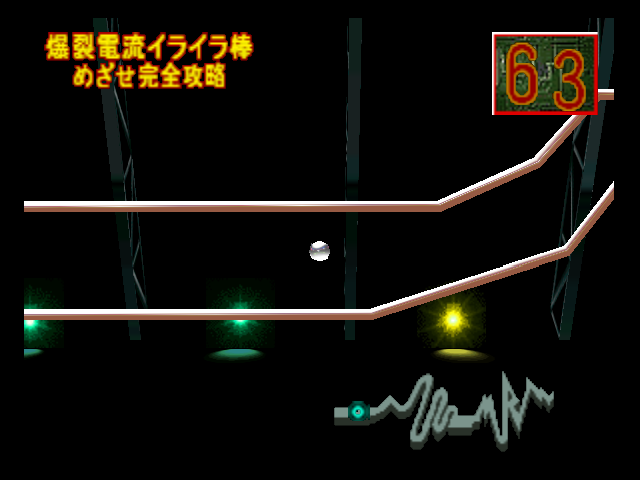
\includegraphics[scale=0.5]{utchan.png}
    \caption{\textit{Denryu Iraira Bou}}
    \label{fig:iraira}
\end{figure}

Have you ever played wire loop games before? It involves guiding a metal loop along a serpentine length of wire without touching the loop to the wire; otherwise you would get an electric shock.

\textit{Miku} is recently obsessed with a similar game called \textit{The Irritating Maze}. Known in Japan as ウルトラ電流イライラ棒 (\textit{Ultra Denryu Iraira Bou}), it is a 2D maze game where players need to guide an electrode ball through a course while avoiding the metallic frame and other moving obstacles (as shown in Figure \ref{fig:iraira}).

After cracking all levels with ease, \textit{Miku} is thinking of something interesting: how large can she change the ball  such that the game is still passable, theoretically? Obviously, when the ball becomes too big it either touches the wall or collides with an obstacle. To increase the ball size, \textit{Miku} needs to wrap some layers of metal to the ball. The in-game editor only provides a range of metal layers, so she has to add them one by one until the ball cannot be larger!

\textit{Miku} has asked you to write a program to help her determine the maximum number of metal layers she can use. Can you help her out?

In two dimensions, the electrode ball can be described as a circle with radius $R$ when nothing is wrapped. She has $N$ metal layers, the $i^\text{th}$ of which has some thickness $t_i$. Using the $i^\text{th}$ layer would increase ball radius by $t_i$. For simplicity, the course can be described as a rectangular box filled with circular obstacles. The rectangle has length $L$ in the East-West direction, and width $W$ in the North-South direction.

\textit{Miku} has to move the ball from the Western end of the labyrinth to the Eastern end without getting shocked, so she must not touch either of the Northern or Southern walls, nor any of the obstacles. She can choose any starting point at the Western end, and any endpoint at the Eastern end.

\textbf{What is the maximum number of metal layers \textit{Miku} can apply to the electrode ball such that she can still pass the game?}

\section{Input}

The first line of input contains two space-separated integers $R$ ($1 \leq R \leq 1,000$) and $N$ ($1 \leq N \leq 10^4$), which corresponds to the ball's initial radius and the number of metal layers available.

The second line contains $N$ space-separated integers, the $i^\text{th}$ of which, $t_i$, is the thickness of $i^\text{th}$ layer ($0 < t_i \leq 100$).

The third line contains three space-separated integers $L$ ($1 \leq L \leq 10^4$), $W$ ($1 \leq W \leq 10^4$), and $M$ ($0 \leq N \leq 2000$): the length of the box, the width of the box, and the number of obstacles, respectively.

The next $M$ lines describe the obstacles. The $i^\text{th}$ line contains three space-separated integers $x_i$ ($0 \leq x_i \leq L$), $y_i$ ($0 \leq y_i \leq W$), and $r_i$ ($0 < r_i \leq 10^4$) indicating that the $i^\text{th}$ obstacle is a circle of radius $r_i$ centered at position ($x_i$, $y_i$) ($x_i$ from the Western wall, and $y_i$ from the Southern wall).

\section{Output}

Display the maximum number of metal layers \textit{Miku} can apply to the electrode ball, between 0 and $N$, inclusive. Display \texttt{-1} if it is not possible.

\section{Samples}

\begin{center}
\def\arraystretch{1.8}%
\begin{tabular}{|p{0.47\textwidth}|p{0.47\textwidth}|}
\multicolumn{1}{l}{\textbf{Sample Input 1}} & \multicolumn{1}{l}{\textbf{Sample Output 1}} \\
\hline
\begin{tabularverbatim}
200 1
10
10000 10000 0
\end{tabularverbatim}
&
\begin{tabularverbatim}
1
\end{tabularverbatim}
\\ \hline
\end{tabular}

\vspace{20pt}

\begin{tabular}{|p{0.47\textwidth}|p{0.47\textwidth}|}
\hline
Sample Input 2 & Sample Output 2\\
\hline
\begin{tabularverbatim}
200 10
5 5 5 5 5 5 5 5 5 5
10000 450 0
\end{tabularverbatim}
&
\begin{tabularverbatim}
4
\end{tabularverbatim}
\\ \hline
\end{tabular}

\vspace{20pt}

\begin{tabular}{|p{0.47\textwidth}|p{0.47\textwidth}|}
\hline
Sample Input 3 & Sample Output 3\\
\hline
\begin{tabularverbatim}
50 10
1 2 3 4 5 6 7 8 9 10
10000 500 1
5000 250 100
\end{tabularverbatim}
&
\begin{tabularverbatim}
6
\end{tabularverbatim}
\\ \hline
\end{tabular}

\vspace{20pt}

\begin{tabular}{|p{0.47\textwidth}|p{0.47\textwidth}|}
\hline
Sample Input 4 & Sample Output 4\\
\hline
\begin{tabularverbatim}
100 3
1 2 3
10000 200 0
\end{tabularverbatim}
&
\begin{tabularverbatim}
-1
\end{tabularverbatim}
\\ \hline
\end{tabular}

\end{center}

\section{Explanations}

\subsection{Sample 1}

% NEED TO DRAW THE RECTANGLE

\begin{center}
\centering
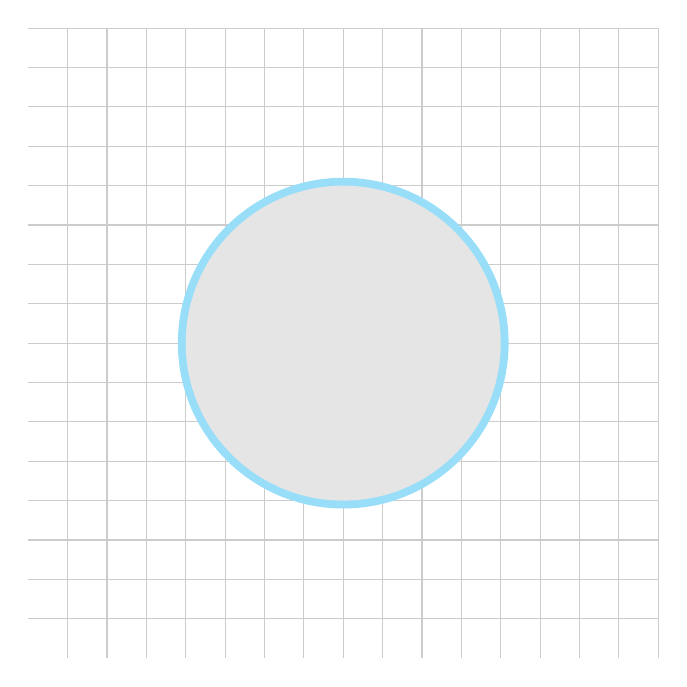
\begin{tikzpicture}
    \draw[step=.5cm,draw=black!20] (46,46) grid (54,54);
	\fill[fill=cyan!40] (50,50) circle (2.1cm);
	\fill[fill=black!10] (50,50) circle (2cm);
\end{tikzpicture}
\end{center}

\subsection{Sample 2}

% NEED TO DRAW THE RECTANGLE + put the largest ball possible

\begin{center}
\centering
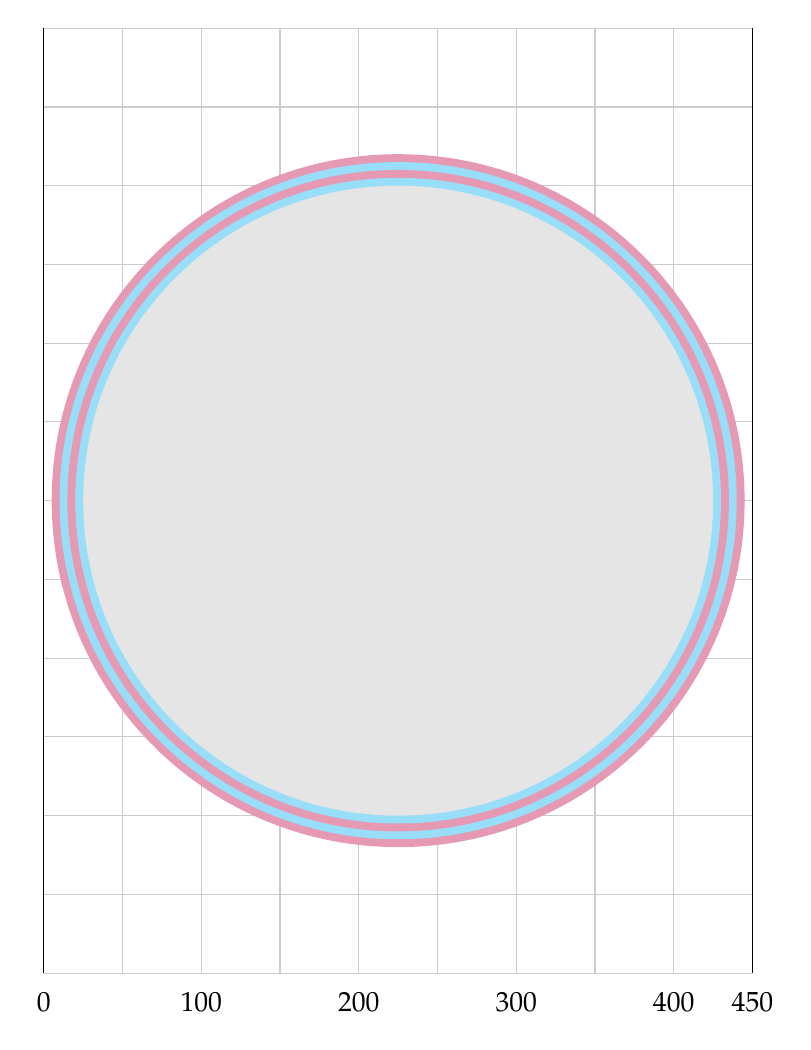
\begin{tikzpicture}[scale=2]
    \draw[step=.5cm,draw=black!20] (0,0) grid (4.5,6);
    \draw (0,0) -- (0,6);
    \draw (4.5,0) -- (4.5,6);
    \fill[fill=purple!40] (2.25,3) circle (2.2cm);
    \fill[fill=cyan!40] (2.25,3) circle (2.15cm);
    \fill[fill=purple!40] (2.25,3) circle (2.1cm);
    \fill[fill=cyan!40] (2.25,3) circle (2.05cm);
    \fill[fill=black!10] (2.25,3) circle (2cm);
    \node at (4.5,0) [label=below:450] {};
    \node at (4,0) [label=below:400] {};
    \node at (3,0) [label=below:300] {};
    \node at (2,0) [label=below:200] {};
    \node at (1,0) [label=below:100] {};
    \node at (0,0) [label=below:0] {};
\end{tikzpicture}
\end{center}

\subsection{Sample 3}

% NEED TO DRAW THE RECTANGLE + put the largest ball possible

\begin{center}
\centering
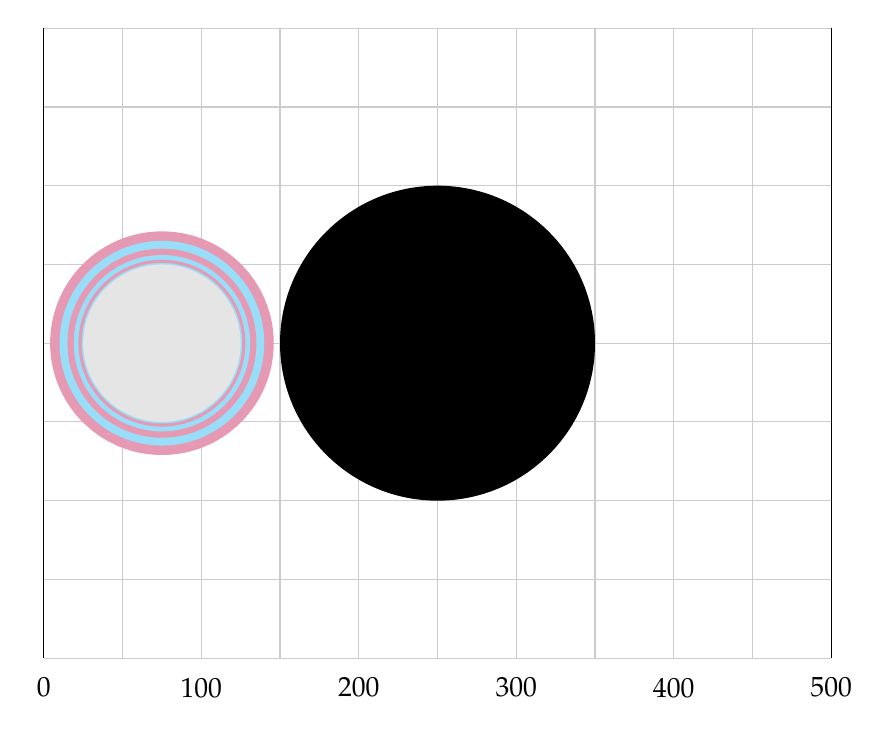
\begin{tikzpicture}[scale=2]
    \draw[step=.5cm,draw=black!20] (0,0) grid (5,4);
    \draw (0,0) -- (0,4);
    \draw (5,0) -- (5,4);
    \fill[fill=black] (2.5,2) circle (1cm);
    \fill[fill=purple!40] (0.75,2) circle (0.71cm);
    \fill[fill=cyan!40] (0.75,2) circle (0.65cm);
    \fill[fill=purple!40] (0.75,2) circle (0.6cm);
    \fill[fill=cyan!40] (0.75,2) circle (0.56cm);
    \fill[fill=purple!40] (0.75,2) circle (0.53cm);
    \fill[fill=cyan!40] (0.75,2) circle (0.51cm);
    \fill[fill=black!10] (0.75,2) circle (0.5cm);
    \node at (5,0) [label=below:500] {};
    \node at (4,0) [label=below:400] {};
    \node at (3,0) [label=below:300] {};
    \node at (2,0) [label=below:200] {};
    \node at (1,0) [label=below:100] {};
    \node at (0,0) [label=below:0] {};
\end{tikzpicture}
\end{center}

\subsection{Sample 4}

% NEED TO DRAW THE RECTANGLE + Put original ball there showing it's gonna touch the wall

\begin{center}
\centering
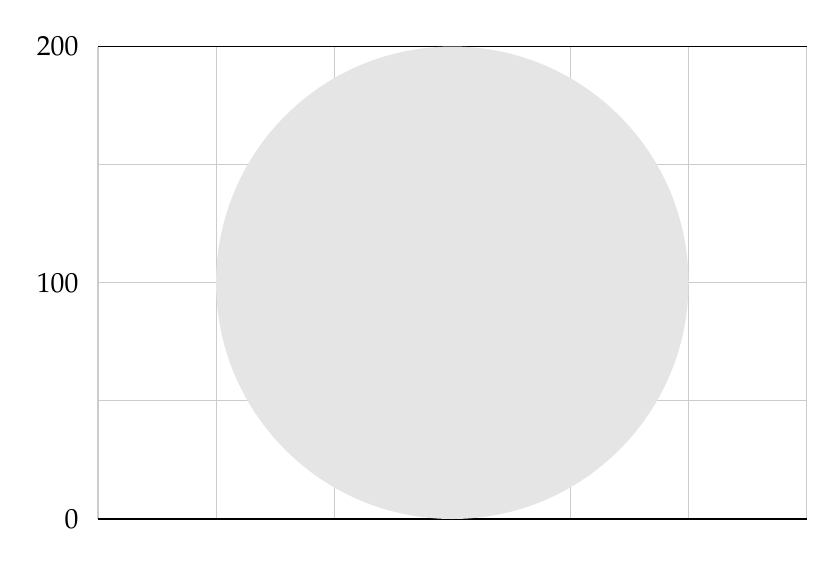
\begin{tikzpicture}[scale=3]
    \draw[step=.5cm,draw=black!20] (0,0) grid (3,2);
    \draw (0,0) -- (3,0);
    \draw (0,2) -- (3,2);
    \fill[fill=black!10] (1.5,1) circle (1cm);
    \node at (0,2) [label=left:200] {};
    \node at (0,1) [label=left:100] {};
    \node at (0,0) [label=left:0] {};
\end{tikzpicture}
\end{center}

\end{document}
